\documentclass{article}
\usepackage[utf8]{inputenc}
\documentclass{article}
\usepackage[utf8]{inputenc}
\documentclass{article}
\usepackage[dvips]{graphicx}
\usepackage{a4wide}
\usepackage{amsmath}
\usepackage{euscript}
\usepackage{amssymb}
\usepackage{amsthm}
\usepackage{amsopn}

\theoremstyle{definition}
\newtheorem*{definition}{Definition}
\newtheorem{theorem}{Theorem}
\newcommand{\cis}{\mbox{cis}}
\newcommand{\vv}{\ensuremath{\vec{v}}}
\newcommand{\vu}{\ensuremath{\vec{u}}}
\newcommand{\vw}{\ensuremath{\vec{w}}}
\newcommand{\vx}{\ensuremath{\vec{x}}}
\newcommand{\vy}{\ensuremath{\vec{y}}}
\newcommand{\vb}{\ensuremath{\vec{b}}}
\newcommand{\vo}{\ensuremath{\vec{0}}}
\newcommand{\va}{\ensuremath{\vec{a}}}
\newcommand{\ve}{\ensuremath{\vec{e}}}

\newcommand{\R}{\mathbb{R}}
\newcommand{\Z}{\mathbb{Z}}
\newcommand{\C}{\mathbb{C}}
\newcommand{\N}{\mathbb{N}}
\newcommand{\Q}{\mathbb{Q}}
\title{Complex Analysis}
\author{ajbergquist }
\date{August 2021}

\usepackage{ulem}
\usepackage{xcolor}
\newcommand{\cs}[1]{\color{blue}{#1}\normalcolor}

\begin{document}
\fbox{notation} Let $\cis\theta$ denote $\cos\theta + i\sin\theta$.\\
\fbox{4a} The third roots of $-1$, $(-1)^{\frac{1}{3}}$. To find these, we convert to exponential form. Since $\arccos(-1) = \pi$, \cs{The arccos command has two cs.} and $|-1| = 1$, we have $-1 = e^{\pi i}.$ Furthermore, using DeMoivre's formula and other stuff, $(-1)^{\frac{1}{3}} = e^{\frac{\pi i}{3}} = \exp(\frac{\pi i}{3} + \frac{2k\pi i}{3})$ for $k = 0,1,2$. Hence we have $\cis(\pi/3) = 1/2 + \sqrt{3}/2 i$, $\cis(3\pi/3) = -1$, $\cis(5\pi/3) = 1/2 - \sqrt{3}/2 i.$ The principle root is $-1$. \cs{The principle root is the one that uses $k=0.$} Drawing this out, we have something like this:
\begin{figure}[htbp]
\centerline{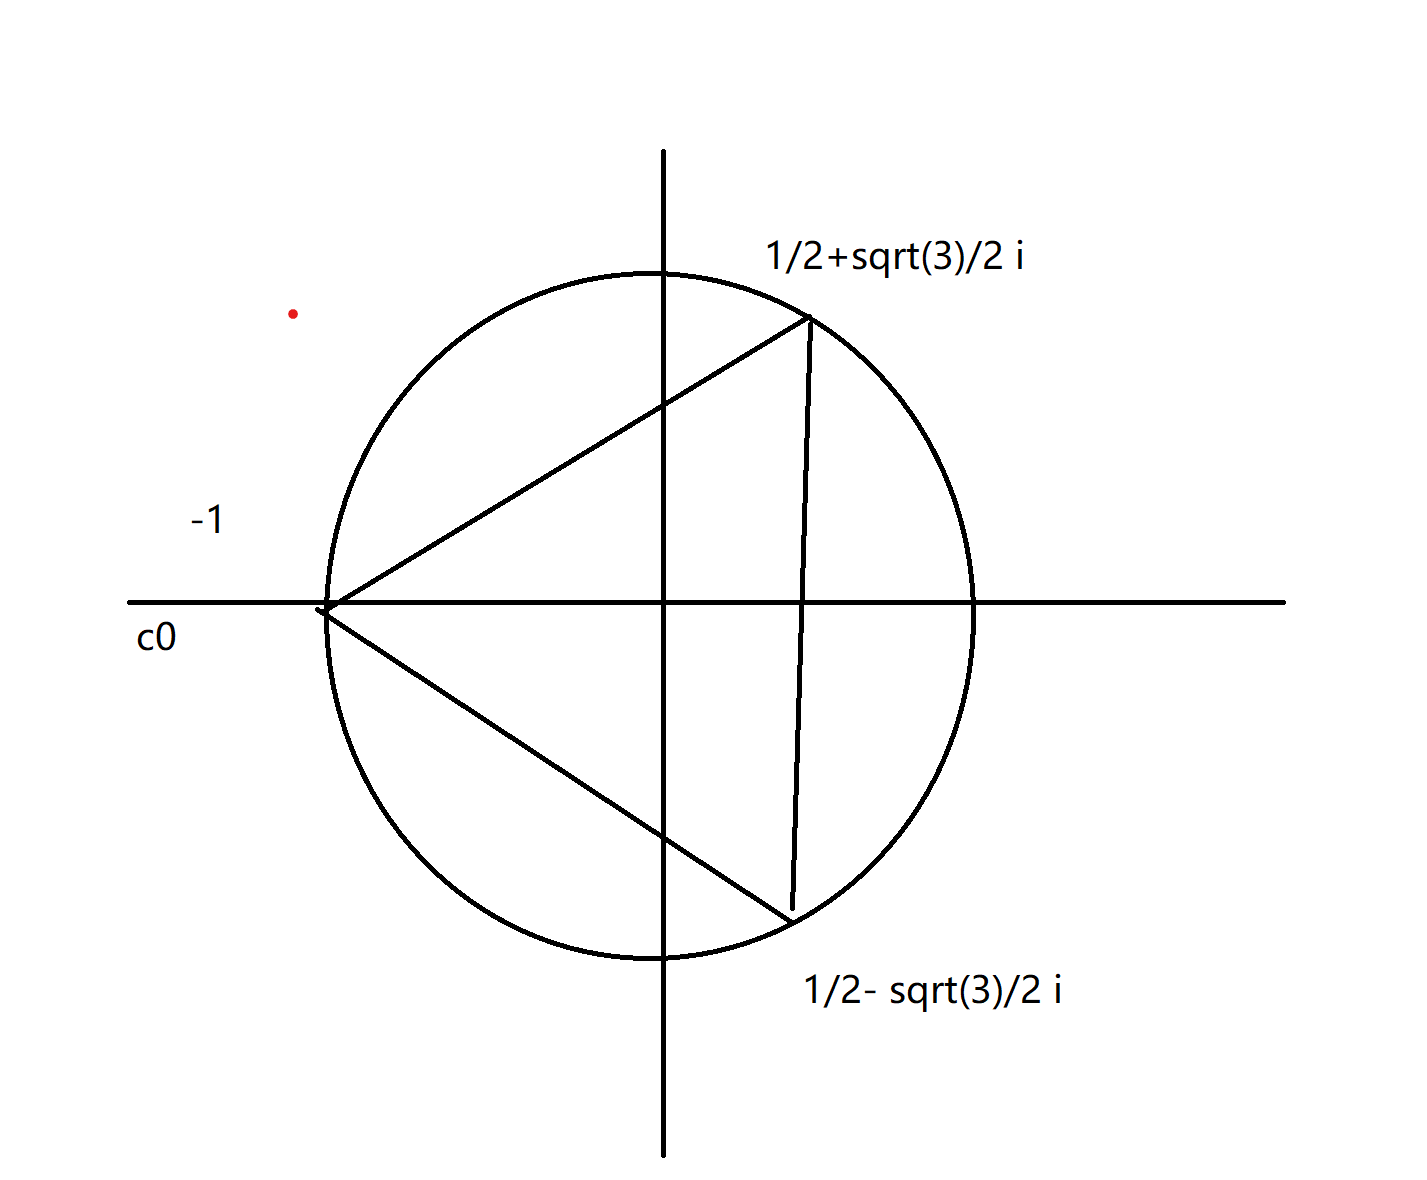
\includegraphics[scale=0.5]{roots-1.png}}
\caption{The third roots of -1}
\label{fig}
\end{figure}\\
\fbox{4b} The sixth roots of $8$, denoted $8^{\frac{1}{8}}$, can be found by first writing $8$ in polar exponential form. Converting, we have $8 = 8\exp(2\pi k i)$ for $k\in \Z$. Using DeMoivre's formula, we derive $$8^{\frac{1}{6}} = \{8^{\frac{1}{6}}\exp(\frac{2\pi k}{2}):k = 0,1,2,3,4,5\}.$$ \cs{$\exp(2\pi ki/6)$?} Computing for each $k$ and using the same trig identities as the last, we get $ $
\begin{figure}[htbp]
\centerline{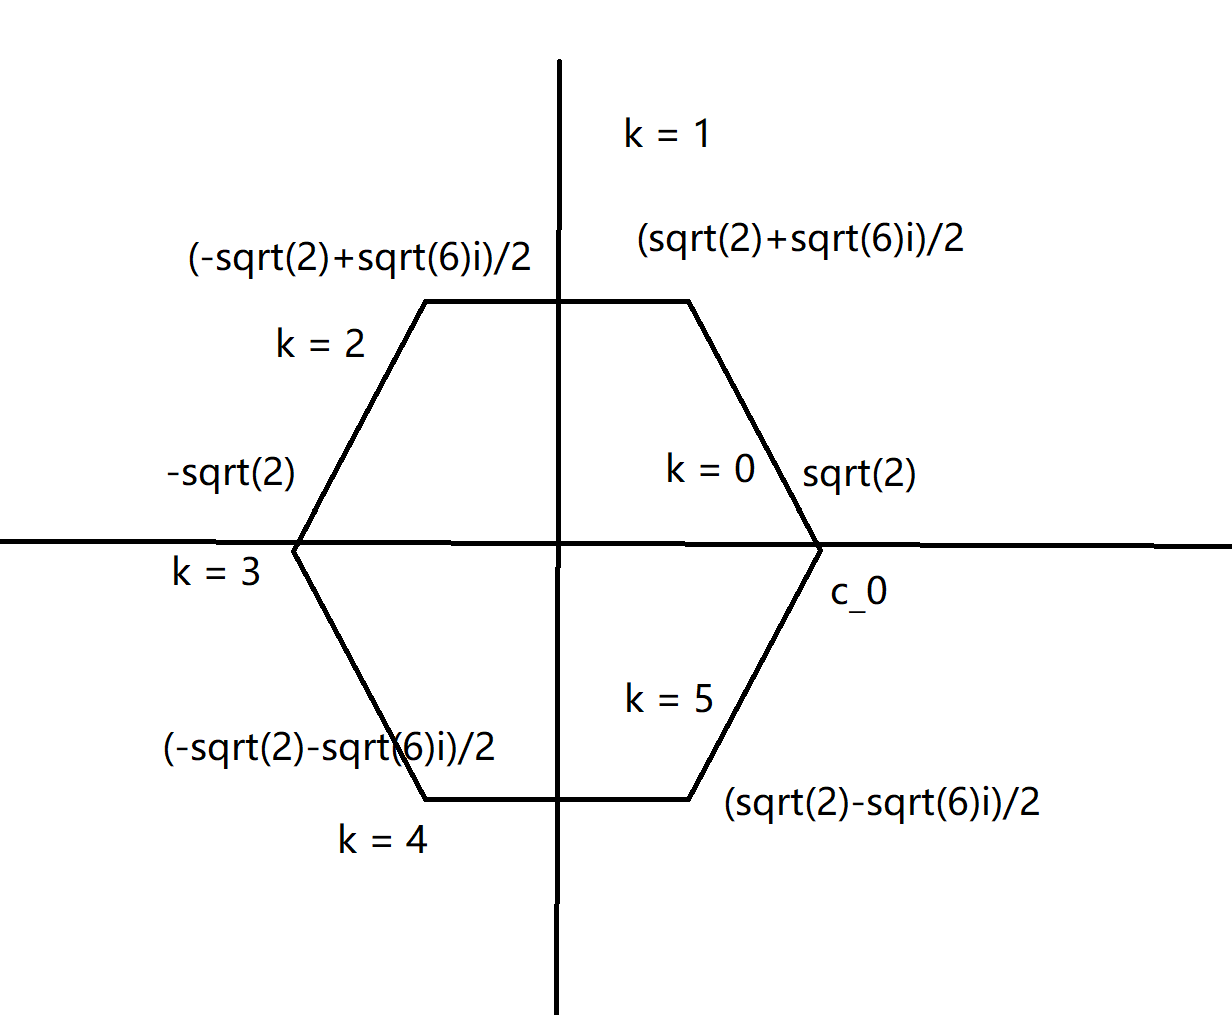
\includegraphics[scale=0.5]{6roots.png}}
\caption{The third roots of -1}
\label{fig}
\end{figure}\\
\\
\cs{I think Figure 2 is mislabeled...}

\fbox{7: proposition} Let $n>1\in \Z$, and let $c$ be an arbitrary $n$th root of unity such that $n \ne 1$. Then $1 + c + c^2+\dots+c^{n-1} = 0$.\\
\fbox{lemma} Before we prove this, we first need to prove something we haven't proven yet. This is the proposition that given any complex number $z\in \C$ and any positive integer $n$, the sum 
$$1 + z +  z^2 + \dots + z^n = \frac{1-z^{n+1}}{1-z}.$$
\fbox{proof for lemma} We proceed by induction. Let $z \ne 0$ be an arbitrary complex number. For the base case, let $n = 1$. Then we have $$\frac{(1 - z)^2}{1-z} =  = \frac{(1+z)(1-z)}{1-z} = 1+z.$$ Hence the base case holds. Now suppose that there exists some positive integer $n$ integer $n$ such that $1+z+z^2+\dots+z^n = \frac{1-z^{n+1}}{1-z}$. Now adding $z^{n+1}$ to the sum, we have by substitution $$\begin{array}{cc}
     &  1+z+z^2+\dots+z^n+z^{n+1} \\
     & = \frac{1-z^{n+1}}{1-z}+z^{n+1}\\
     & = \frac{1-z^{n+1}+z^{n+1}(1-z)}{1-z}\\
     & = \frac{1-z^{n+1}z}{1-z} = \frac{1-z^{n+2}}{1-z}.
\end{array} $$
Hence by way of induction, the proposition holds for all positive integers $n$.\\

\cs{It would be okay to take this as previously proven. (But nice job!} 

\fbox{proof} Having proven this result, the proof follows easily. Let $n$ be an arbitrary natural number greater than $1$, and let $c$ be an $n$th root of unity not equal to $1$. Since the roots of unity all have the form $\exp(\frac{2k\pi}{n})$, \cs{Remember the $i$!} we can write $c = \exp(\frac{2k\pi}{n})$ for some arbitrary $k = 1,\dots,n-1$. ($k\ne 0$ because $c$ is explicitly not $1$). Furthermore, since $c$ is a nonzero complex number, we an apply the lemma to attain the result 
$$1+ c + \dots+ c^{n-1} = \frac{1-c^{n}}{1-c} = \frac{1-[\exp([n2k\pi/n = 2k\pi])= 1]}{1-c} = 0.$$\\

\cs{Without the $i$, this is false, so keep it in mind as you go.}
\cs{oh yeah, oops!}

\cs{5/5}

\cs{10/10}

\fbox{9: proposition} Any complex number in a domain is an accumulation point. In this proof, the epsilon-neighborhood of $z$ is denoted $N_\epsilon(z) = \{z_0:|z-z_0|<\epsilon\}$. The deleted epsilon-neighborhood of $z$ is denoted $D_\epsilon(z) = N_\epsilon(z) - \{z\}$\\

\fbox{lemma} Let $0<\epsilon\in \R$ and $z\in \C$, and let $\delta>\epsilon \in \R$. Then $D_\epsilon(z) \subseteq D_\delta(z)$.\\
\fbox{proof} If $D_\epsilon(z)$ is empty (which it can't be), then the proposition holds. Assume then that it isn't. Let $z_0$ be an arbitrary element in $D_\epsilon(z)$. Then we have by definition of a deleted neighborhood $0<|z-z_0|< \epsilon$. By substitution, $0<|z-z_0| < \epsilon < \delta$, hence by definition of $D_\delta(z)$, $z\in D_\delta(z)$. \cs{Wait! By definition, $z$ is {\bf not} in $D_{\epsilon(z)}$!} Since $z$ is arbitrary, $D_\epsilon(z) \subseteq D_\delta(z).$\\ \cs{Did you mix up your $z$ and $z_0$?} \cs{oh, yeah that's definitely what happened}



\fbox{actual proof} Let $S$ be a domain, and let $z$ be an arbitrary element in $S$. Since $z$ is an element in a domain, it follows by a previously proven theorem that $z$ is an interior point of $S$. By definition of an interior point, there exists some epsilon neighborhood of $z$, $N_\epsilon(z)$, for some $\epsilon > 0$, such that $N_\epsilon(z)$ is a subset of $S$. Since $D_\epsilon(z)$ is is a subset of $N_\epsilon(z)$, it follows that $D_\epsilon(z)$ is a subset of $S$. Since no deleted neighborhood of $z$ can be empty, it follows that there exists an element $z_0\in D_\epsilon(z)$. \\
Let $\delta$ be an arbitrary real number greater than $\epsilon$. By the lemma, it follows that $D_\epsilon(z)\subseteq D_\delta(z)$, hence $z_0\in D_\delta(z)$. Since $\delta$ is arbitrary, it follows that for all real numbers $\delta$ greater than $\epsilon$, $z_0\in D_\delta(z)$ and $z_0\in S$. Since for any "epsilon" less than $\epsilon$ the deleted neighborhood of $z$ must be a subset of $D_\epsilon(z)$, it follows in any of these cases that there is some element of all of these deleted neighborhoods in $S$. Since all epsilon less and greater than $\epsilon$ include all positive real numbers, it follows that for any deleted neighborhood of $z$ there is a point also in $S$. Hence $z$ is an accumulation point of $S$. Since $z$ and $S$ are arbitrary, it follows that for any domain $S$, each point in $S$ is an accumulation point of $S$. 

\cs{5/5}

\end{document}
